\chapter{Desenvolvimento do Projeto}

Neste capítulo é abordado tudo o que foi necessário para chegar em um projeto viável, como tecnologias utilizadas, arquitetura do sistema, viabilidade financeira, critérios necessários para segurança da aplicação, casos de uso e regras de negócio como também métricas para dimensionar dificuldades, qualidade e tamanho do aplicativo.   



\section{Arquitetura do sistema}
O aplicativo em React Native será provisionado na loja de aplicativos do Android, PlayStore, e, a partir do momento em que o usuário efetuar o download desse e estiver conectado à internet, o aplicativo se comunica com os servidores da Google para efetuar a autenticação social com o Google via OAuth 2.0. 

E, devido a uma eficiente integração com a plataforma Node.js., a plataforma Heroku foi a escolhida para provisionar em produção a API que será consumida pelo front-end, como mostrado na \autoref{arquitetura-sistema}. Essa API (Application Programming Interface) é a responsável por receber as requisições do aplicativo e comunicar-se com outras duas aplicações: a primeira é o banco de dados MongoDB, hospedado em produção na plataforma de nuvem MongoDB Atlas - a qual foi desenvolvida exclusivamente para hospedar esse banco de dados não relacional -, e a segunda aplicação trata-se do Cloudinary, uma CDN (Content Delivery Network) que, nesse primeiro momento, será utilizada para armazenar as fotos de perfil dos usuários cadastrados no aplicativo.


\begin{figure}[htb]
	\centering
	\caption{\label{fig_arq_virado}Arquitetura do sistema}
	\label{arquitetura-sistema}
	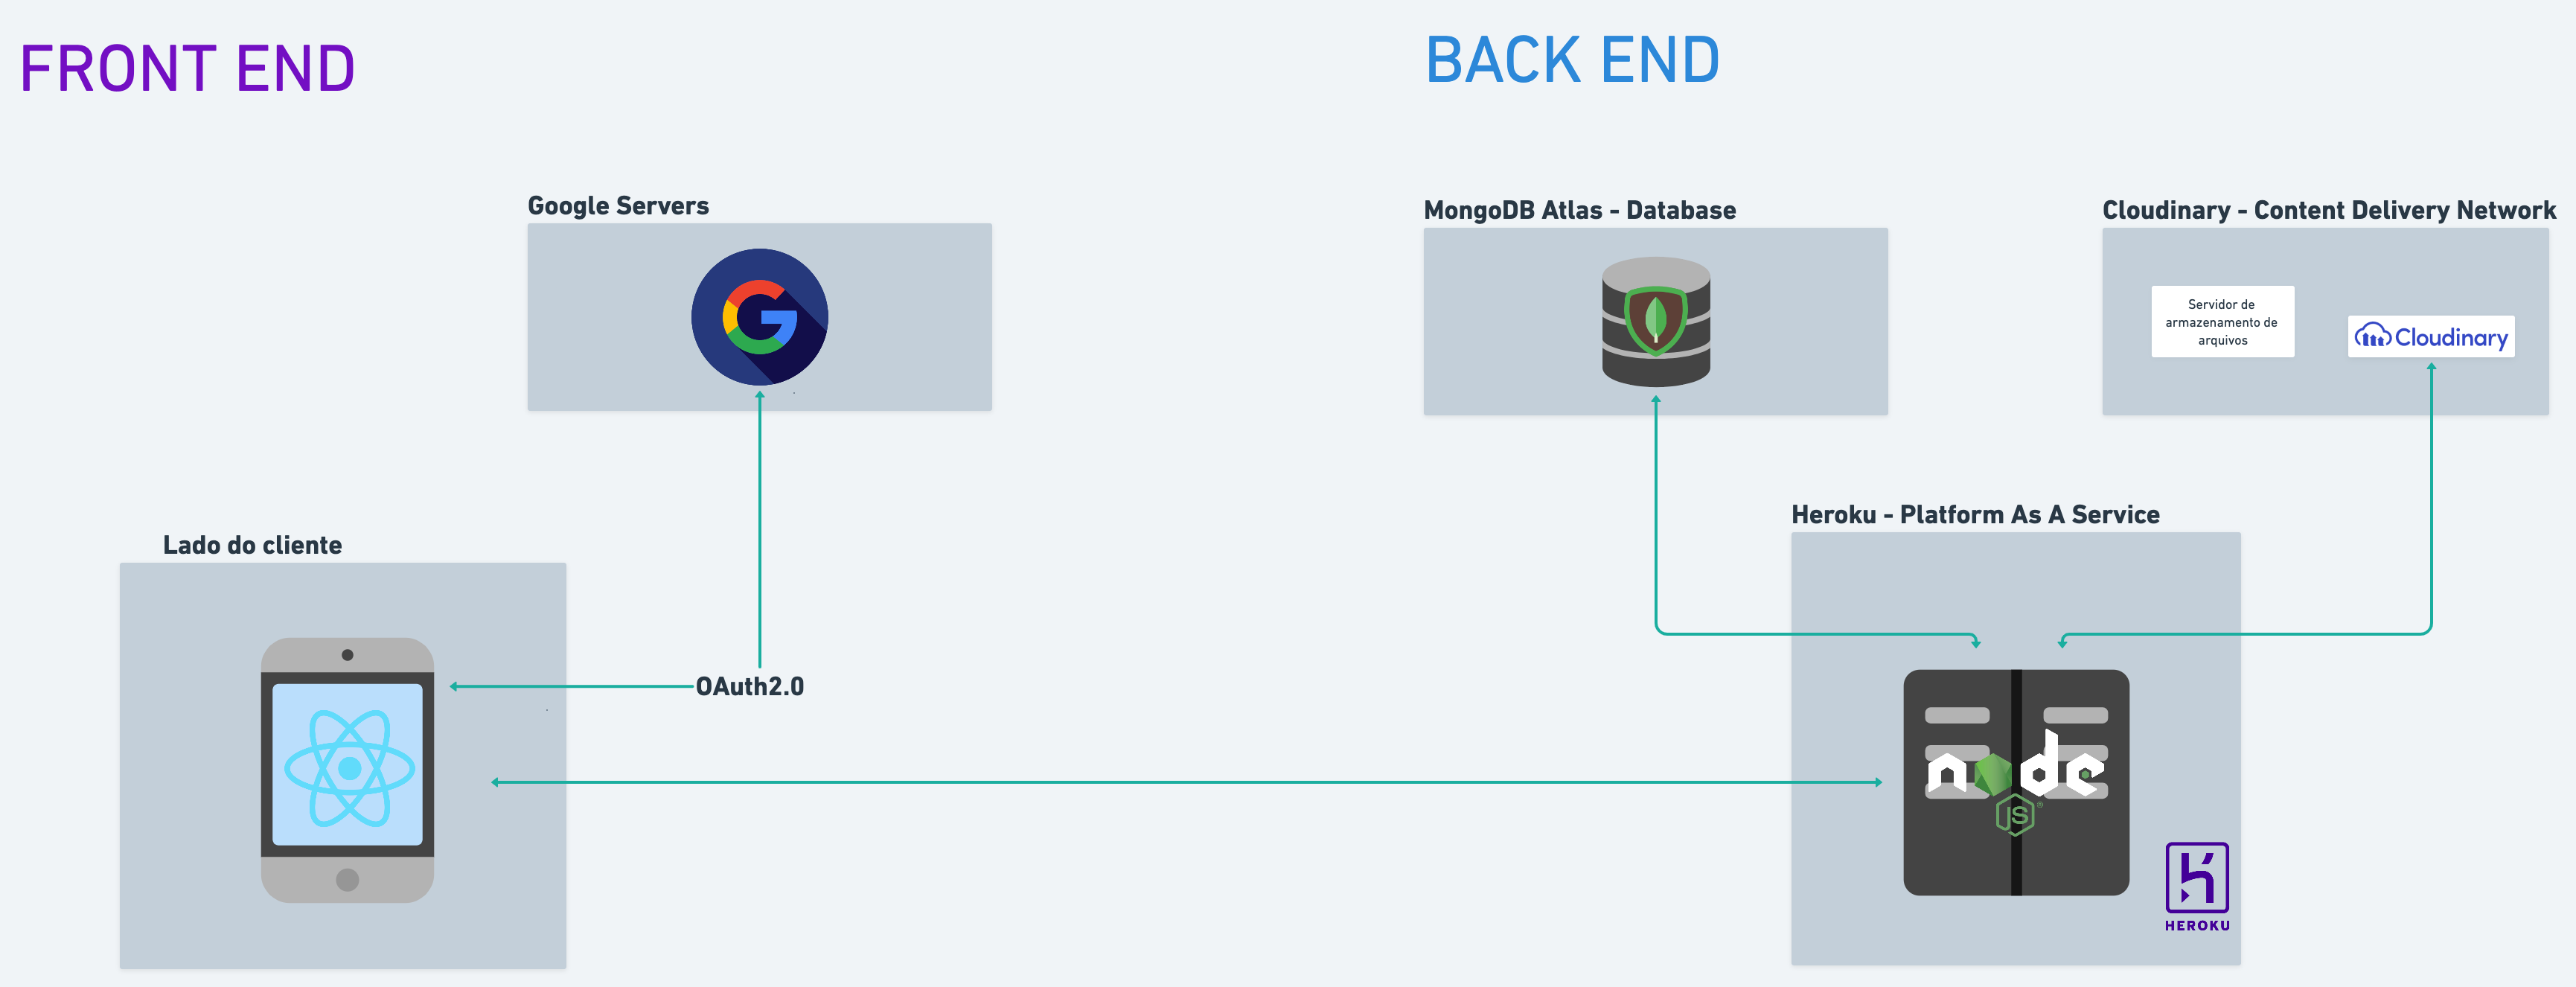
\includegraphics[width=0.9\textwidth]{anexos/poc-arquitetura.png}
	\fonte{Equipe diversaGente (2022)}
\end{figure}


\section{Motivação para a escolha da plataforma Android}
A empresa data.ai, que utiliza Ciência de Dados para analisar o mercado mobile em todo o mundo, divulgou um relatório que demonstra que o Brasil é líder na utilização de smartphones. A população brasileira passa, em média, 5,4 horas diárias consumindo conteúdos pelo celular, enquanto a média global é de 4,8 horas \cite{stateof}.
PER
Somente em 2021, foram lançados 2 milhões de aplicativos móveis, de acordo com o mesmo relatório da data.ai. Diante dessa massiva demanda por aplicativos móveis, é crescente a busca dessa indústria por soluções que abarquem diversas áreas da vida da população de forma simples e eficiente. 

Como resultado, existem hoje ferramentas de código aberto de alta qualidade que possibilitam a construção de aplicativos intuitivos, acessíveis e escaláveis, tornando a entrega de novas soluções mais rápidas e fáceis às equipes de software. 

Então, dado o sucesso dos aplicativos na atualidade, foi escolhido construir o aplicativo diversaGente devido a possibilidade de utilizar práticas e ferramentas bem estabelecidas no mercado e assim alcançar um número expressivo de usuários dentro de uma área aquecida e em expansão.

O foco atual é a um aplicativo otimizado para o Android, sistema operacional amplamente utilizado no Brasil e que, de acordo com relatório de 2020 Impacto econômico e social do Android no Brasil, da consultoria digital Bain & Company, é uma plataforma que teve impacto decisivo para o acesso à internet de milhares de brasileiros. Portanto, diante do forte objetivo de inclusão do aplicativo, o foco no Android contribui para tal.
Assim, após a escolha do tipo de aplicação a ser construída, foram elencadas as ferramentas para o desenvolvimento back-end e front-end. 


\section{Escolhas das tecnologias para o back-end}
Para a construção back-end desse aplicativo, são necessários necessários serviços, processos, persistência dos dados e uma interface. Então para atender essas necessidades, foi escolhida uma Stack amplamente utilizada e bem estabelecida na indústria conhecida como MERN, a qual supre a necessidade do contexto do aplicativo diversaGente. 
MERN refere-se a um conjunto de tecnologias utilizado para o desenvolvimento de aplicações, sendo, respectivamente, a base de dados não relacional MongoDB, um módulo minimalista de roteamento chamado Express.js, um framework desenvolvido pelo Facebook baseado em React mencionado na seção seguinte sobre as tecnologias do front-end,  o React Native, e, por fim, o Node.js, um executor de Javascript no lado do servidor para criação de aplicações que executam no servidor como APIs.

Nesse contexto, ainda se faz necessário provisionar o ambiente local para os desenvolvedores atuarem, bem como documentar e testar a aplicação desenvolvida. Então, para lidar com o ambiente em máquinas de diferentes sistemas operacionais, os containers Docker foram escolhidos, pois provêm alta descartabilidade e reprodutibilidade do ambiente de desenvolvimento e contribuem com menor tempo de configuração local. 

Ainda considerando a eficiência, a existência de uma API bem documentada contribui para um desenvolvimento com menos ruído de informação, então, foi escolhida a especificação OpenAPI, também conhecida como especificação Swagger, para documentar os recursos da API. E, com o objetivo de atingir alta confiabilidade do código back-end, optou-se pelo uso do framework de testes Jest no desenvolvimento.

Junto disso, a escolha de comunicação entre cliente e servidor foi de ocorrer por meio de requisições HTTP (Hypertext Transfer Protocol) para comunicação síncrona por meio de uma API Restful e Websockets, ideal para comunicação em tempo real, necessária no chat que haverá dentro do aplicativo. 
Além disso, foi escolhido o protocolo de autorização OAuth2.0 para a autenticação social do usuário com uma conta do Google, pois, frente ao Firebase inicialmente considerado, esse é um recurso mais simples e enxuto de ser implementado, permitindo que os desenvolvedores dediquem menos tempo em configuração e assim possam investir mais tempo desenvolvendo o que agrega maior valor ao usuário final. Por fim, foi determinada a integração com as APIs do Google Maps para implementação das funcionalidades que envolvem geolocalização. 


\section{Escolhas das tecnologias para o front-end}
Para auxiliar o desenvolvimento da interface a partir de um  protótipo, foi escolhida a ferramenta Figma, editor colaborativo online de design gráfico que permite a criação de interfaces de alta fidelidade e que ajuda desenvolvedores a construir telas coesas. Com essa ferramenta, é almejado alcançar produtividade na construção da interface a partir de um layout pré-definido, poupando decisões de design junto às implementações de código.

E, para obter acesso às APIs nativas do Android, foi escolhida a ferramenta Expo por ela tornar desnecessária a instalação de distintas bibliotecas para acesso aos recursos nativo do smartphone como a localização do dispositivo, câmera e microfone. Dessa forma, diminui-se o número de dependências as quais os desenvolvedores precisam se atentar acerca de grandes atualizações, descontinuamento ou depreciação, bem como possíveis incompatibilidades.

Além disso, o framework de desenvolvimento front-end mobile React Native, baseado em React, foi o escolhido por contar com uma comunidade de desenvolvedores ativos, os quais disponibilizam uma ampla gama de frameworks e outras bibliotecas que podem ser usadas de forma combinada e que provêm soluções bem estruturadas para lidar com questões comuns ao desenvolvimento front-end no geral, como, por exemplo, requisições a APIs, roteamento entre telas e estilização.

Além disso, o React é multiplataforma, o que facilita uma possível expansão do aplicativo em versões futuras para a web bem como para uma adaptação para ser otimizado também ao sistema operacional iOS.
Por fim, para a construção de um layout moderno e que segue boas práticas de UI (User Interface), foi escolhida a biblioteca Native Base, a qual é voltada para a construção de interfaces com o React Native.

\section{Testes automatizados e análise estática}
A fim de garantir uma boa manutenibilidade do código desenvolvido, buscou-se a adoção de um framework de testes automatizados voltado ao ecossistema JavaScript que cumprisse três principais requisitos: o primeiro, receber atualizações rotineiras de melhoria pela equipe de desenvolvimento, o que contribui para  diminuição das chances de que a ferramenta torne-se depreciada em pouco tempo; o segundo, não possuir uma curva de aprendizado muito longa, para facilitar o aprendizado dos conceitos de testes automatizados pelos integrantes do grupo ao passo que os testes são construídos por esses, ou seja, que não demande muito estudo teórico anterior à prática, e terceiro, que gere relatórios de cobertura de código de forma visual e que facilite a interpretação do status de cobertura. 

Diante desses pré-requisitos, foi escolhida a ferramenta de testes automatizados Jest, que conta com uma comunidade ativa, é escrito em JavaScript (linguagem de conhecimento da maioria dos membros da equipe) e que gera páginas HTML com a cobertura de linhas de código de forma visual. 

Já para a análise estática do código, a ferramenta escolhida foi o ESLint, o qual também foi desenvolvido em JavaScript, possui integrações com a maioria das IDEs (Integrated Development Environment) e é utilizada, hoje, por grandes empresas como Airbnb e American Express. E a especificação utilizada é a especificação padrão que a ferramenta já fornece após configuração na aplicação, a qual conta com sugestões para correção de sintaxe, possíveis problemas de lógica e formatação do layout do código, além de oferecer a possibilidade de ser configurado no fluxo de CI/CD (Continuous Integration/Continuous Delivery). 


\section{Sistemas de logs e processo de Integração Contínua}
A plataforma de hospedagem Heroku recomenda algumas ferramentas e serviços que podem ser integrados junto aos aplicativos lá hospedados, e um deles chama-se SolarWinds® Papertrail™. Esse serviço foi escolhido pois, além da fácil integração, oferece uma coleta em tempo real dos logs da aplicação e permite que mensagens de log sejam analisadas de forma simples através de um console acessado pelo navegador, tal como o que é oferecido pela Amazon Web Services (AWS), o que facilita aos desenvolvedores a análise de possíveis problemas e identificação de tendências dos usuários dentro da plataforma como, por exemplo, a que horas geralmente ocorre um pico de usuários ativos.

Já para o processo de integração contínua, importante para garantir que o aplicativo não chegue com falhas à produção, foi estabelecido um fluxo de CI/CD por meio das Github Actions. Para o status atual do projeto, foi estabelecido um fluxo de trabalho executado sempre antes de a API em Node.js ser atualizada em ambiente de desenvolvimento e de produção no Heroku que engloba a preparação do container que receberá as atualizações, download do código atualizado, setup do Node.js, instalação das dependências, execução dos linters, deploy na plataforma Heroku e encerramento dos processos após conclusão do deploy.


\section{Design patterns pertinentes à aplicação}
Por padrão, o React, utilizado no front-end do aplicativo, possui a presença de Injeção de 
Dependência devido a utilização dos arquivos do tipo JavaScript XML (JSX). A utilização de JavaScript junto ao HTML permite a renderização de elementos injetados como componentes, além da utilização de props, que também oferecem a possibilidade de injetar dependências. 

Além disso, existe tanto no back-end quanto no front-end a utilização do padrão Singleton para compartilhar a instância dos serviços, classes e objetos literais. Dessa forma, pode-se garantir a coesão dos dados que serão enviados ao banco de dados no momento em que uma operação for disparada no sistema, como, por exemplo, o cadastro do usuário ou a busca de uma localização específica.


%\pagebreak

\section{Diagramas do sistema}

Nesta seção possui todos os diagramas criados do sistema, para facilitar o entendimento e desenvolvimento da aplicação. 

O diagrama de casos de uso  \autoref{diagrama-caso-uso} foi apresentado na primeira parte da execução do projeto, que foi verificado possíveis utilizações do usuário no sistema. A imagem se encontra no \autoref{diagrama-casos-uso-old}

Como houveram mudanças de escopo para a utilizações do usuário junto a aplicação foi visto a necessidade de criar um novo diagrama de casos de uso conforme a \autoref{diagrama-caso-uso-novo}



\pagebreak

\begin{figure}[htb]
	\centering
	\caption{\label{fig_arq_virado}Diagrama de caso de uso}
	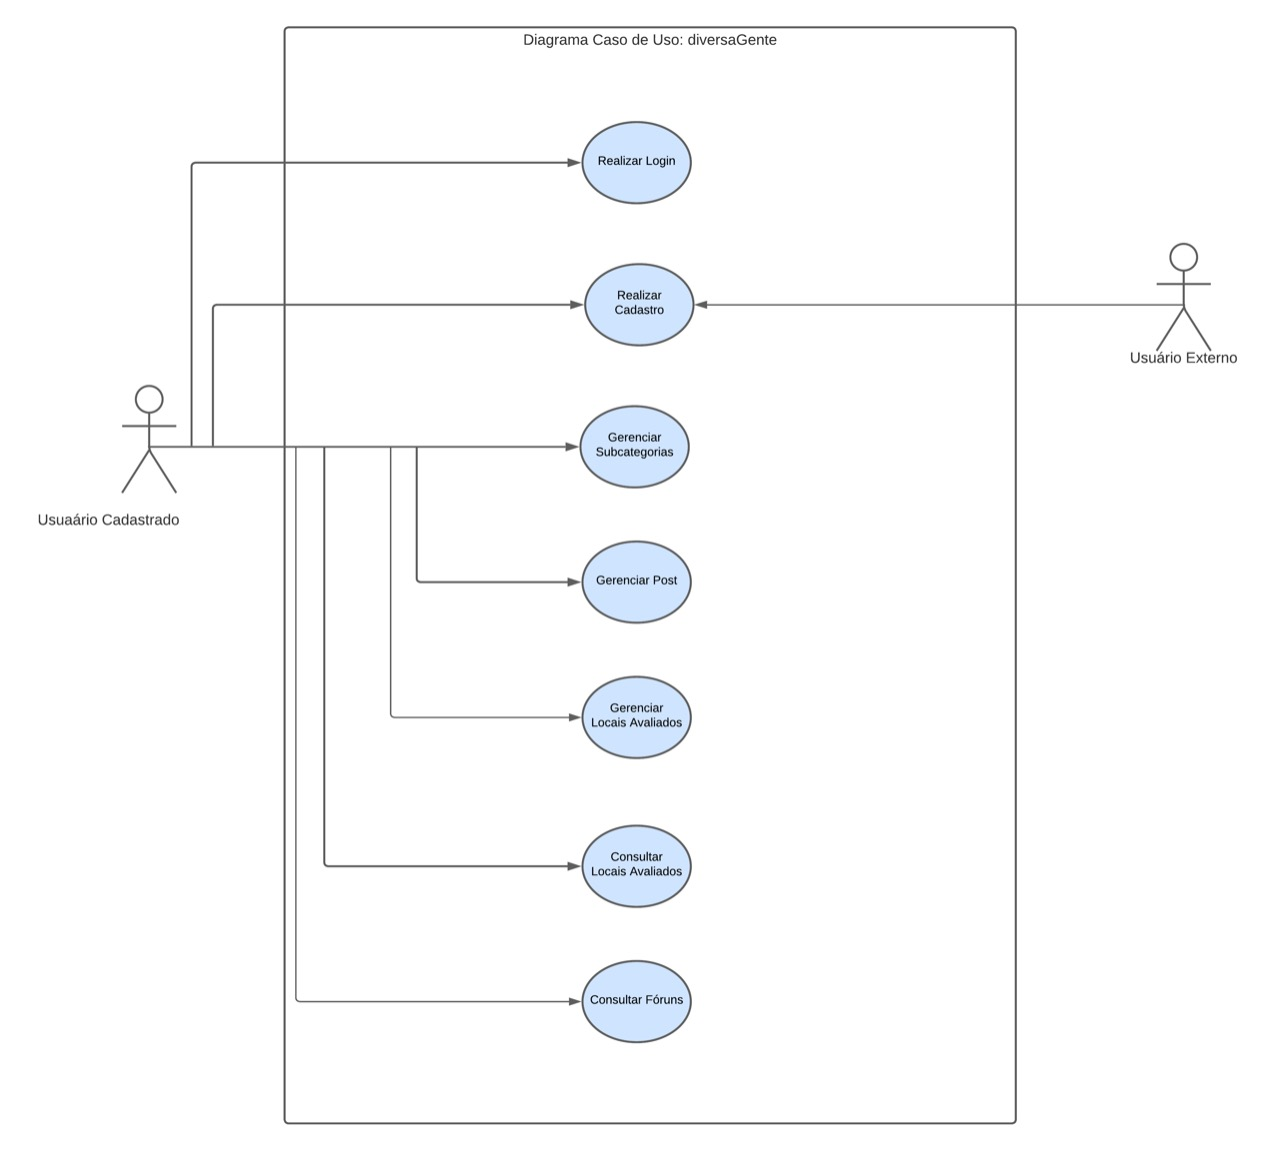
\includegraphics[width=0.90\textwidth]{anexos/Casos de uso.jpeg}
	\label{diagrama-caso-uso-novo}
	\fonte{Equipe diversaGente (2022)}
\end{figure}



As especificações de casos de uso informam através de texto a utilização do usuário ou administrador dentro da aplicação. São identificadas através de códigos que se iniciam com UC, indo do
UC01 \autoref{casos-de-uso1} até o UC21 do \autoref{casos-de-uso21}. Os textos podem ser encontrados no \autoref{casos-de-uso-especificacao}

Após as definições das tecnologias a serem utilizadas e desenho das funcionalidades esperadas na aplicação, foi modelado o Diagrama de Classes conforme presente na \autoref{diagrama-classe} com o objetivo de estabelecer uma boa performance e bom relacionamento entre as entidades do sistema. 
Dentro do aplicativo diversaGente, tem-se a classe User como a principal, pois essa representa o usuário que está atrelado a grande parte das demais classes, como a classe de Posts, Review e Chat, as quais possuem dependência direta da existência do usuário no sistema para que também existam. 

\begin{figure}[htb]
	\centering
	\caption{\label{fig_arq_virado}Diagrama de classes do sistema}
	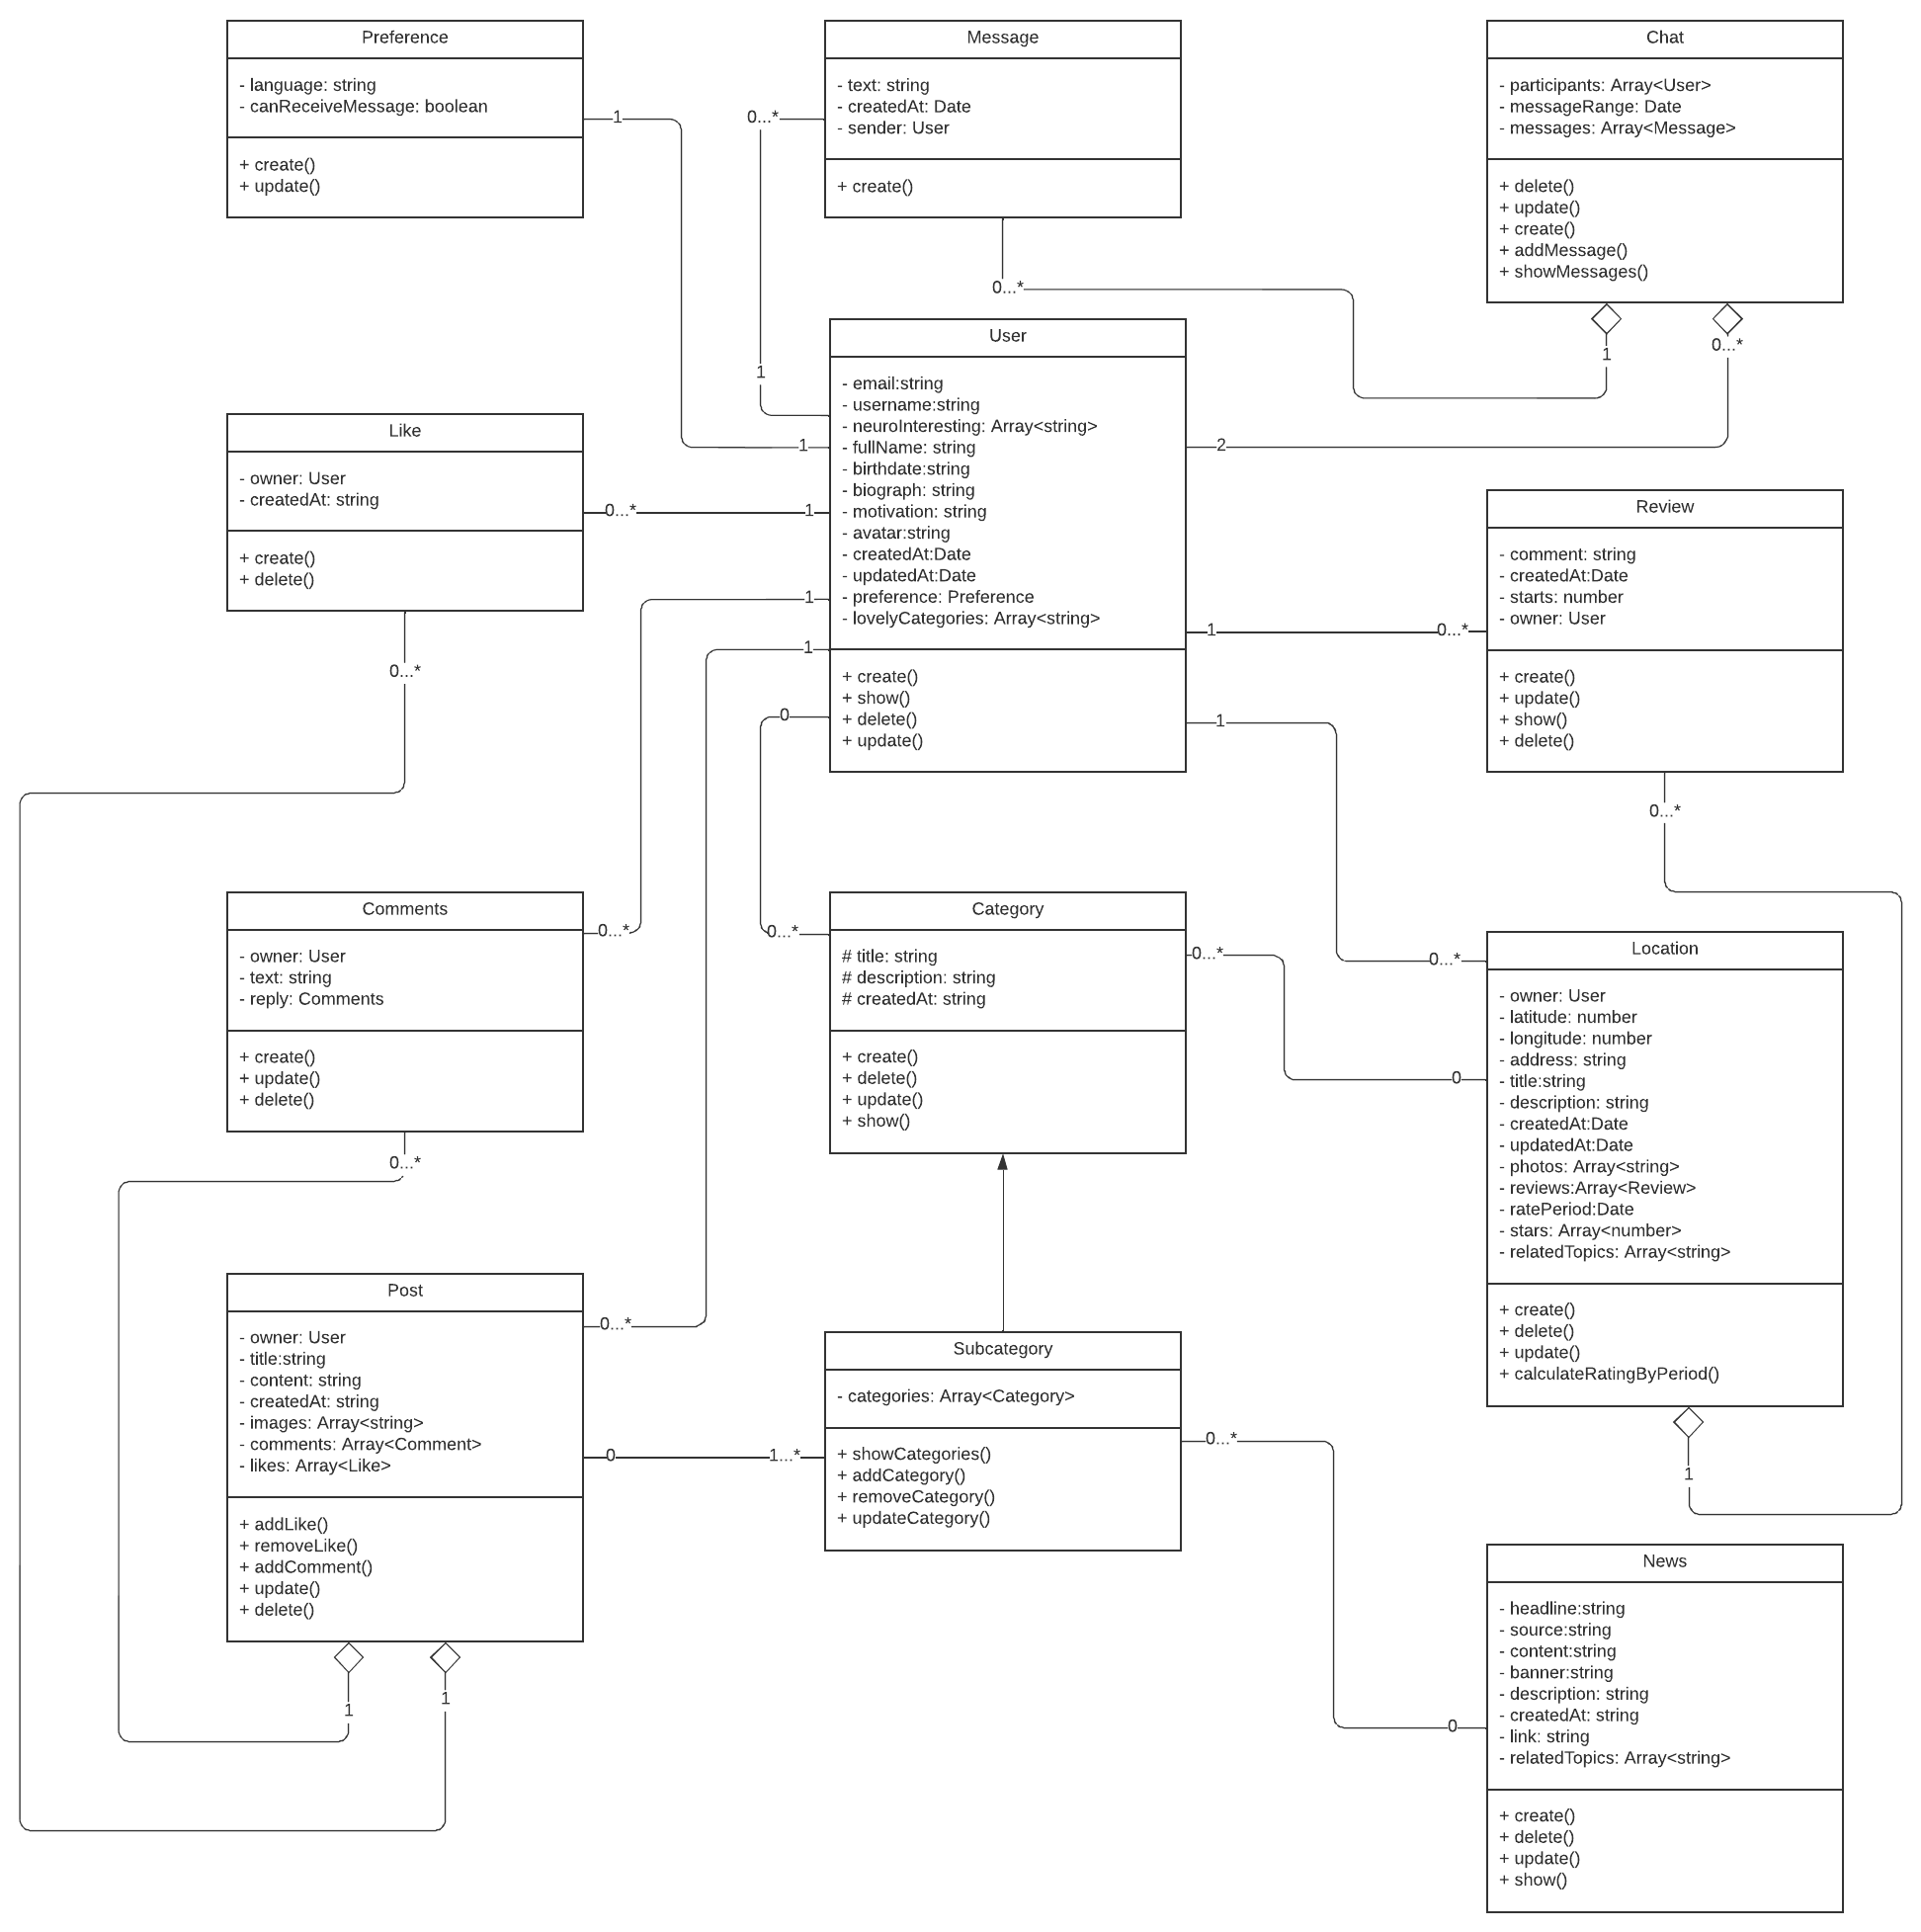
\includegraphics[width=0.90\textwidth]{anexos/diversaGente_-_Classe_UML_1.png}
	\label{diagrama-classe}
	\fonte{Equipe diversaGente (2022)}
\end{figure}

%---------------------------------------------------------------------------------------
\section{Requisitos Funcionais, Não Funcionais e Regras de Negócios}


A análise de requisitos do aplicativo está relacionada com as funcionalidades do sistema e com as prioridades diretamente ligadas a ele. Abaixo, eles estão divididos com suas respectivas funções que englobam tantos os requisitos funcionais, ou seja, declaração dos comportamentos que o sistema deve ter e os requisitos não funcionais que são as restrições colocadas sobre como o sistema deve realizar seus requisitos.

O  \autoref{tabela-requisitos-funcionais} mostra os requisitos funcionais  enquanto a \autoref{requisitos-nao-funcionais} mostra os requisitos não funcionais. 

Para as regras de negócio, \autoref{regra-negocio}, são úteis para definir como as ações vão agir em relação aos processsos da aplicação. 



\begin{quadro}[htb]
	\centering
	\ABNTEXfontereduzida
	\caption[Requisitos Funcionais]{Requisitos Funcionais}
	\label{tabela-requisitos-funcionais}
\end{quadro}
\begin{longtable}{|p{2.0cm}|p{6.5cm}|p{6.5cm}|}
	\hline
	\thead{Código} & \thead{Requisito}  & \thead{Descrição} \\
	\hline
	RF01 & Gerenciar subcategorias. &
	O usuário consegue criar uma nova subcategoria dentro de uma categoria.
	O usuário que criou a subcategoria consegue editar o título das categorias criadas.
	O usuário consegue excluir a categoria que foi criada, recebendo um aviso se realmente é aquilo que ele deseja fazer.
	\\
	\hline
	RF02 & Gerenciar publicações.   & O usuário consegue criar uma nova publicação em uma subcategoria. 
	O usuário consegue editar uma nova publicação dentro de uma subcategoria. 
	O usuário consegue excluir uma publicação dentro de uma subcategoria\\
	\hline
	RF03 & Publicar comentários post  & O usuário consegue comentar em cada publicação. O usuário consegue excluir o comentário em cada publicação. \\
	\hline
	RF04 & Compartilhar imagem dentro das publicações de subcategorias dos fóruns criados &
	O usuário consegue compartilhar as imagens em cada publicação. O usuário consegue excluir as imagens compartilhadas em cada publicação.\\
	\hline
	RF05 & Compartilhar nos aplicativos compatíveis as postagens das subcategorias de discussões dos fóruns criados.  & O usuário deve conseguir compartilhar as postagens com os aplicativos compatíveis.\\
	\hline
	RF06 & Favoritar posts dentro das subcategorias de discussões dos fóruns criados. & O usuário deve conseguir favoritar as mensagens. \\
	\hline
	RF07 & Gerenciar Locais Avaliados. & O usuário deve conseguir cadastrar, editar e excluir um local. O usuário deve conseguir filtrar locais mais próximos do local que se encontra ou de um endereço desejado. \\
	\hline
	RF08 & Permitir que o usuário se cadastre na plataforma. & O usuário deve conseguir criar um cadastro através de login social do google.\\
	\hline
	RF09 & Gerenciar Perfil.  &
	O usuário deve conseguiralterar os seus dados através de uma página de perfil.  \\
	\hline
\end{longtable}
\fonte{Equipe diversaGente (2022)}

\begin{quadro}[htb]
	\centering
	\ABNTEXfontereduzida
	\caption[Requisitos Não Funcionais]{Requisitos Não Funcionais}
	\label{requisitos-nao-funcionais}
	\begin{tabular}{|p{2.0cm}|p{6.5cm}|p{6.5cm}|}
		\hline
		\thead{Código} & \thead{Categoria}  & \thead{Requisito} \\
		\hline
		RNF01 & Compatibilidade &
		Deve ser compatível com o sistema operacional Android.\\
		\hline
		RNF02 & Disponibilidade & O sistema deve estar disponível 24 horas por dia, 7 dias por semana, com tolerância de 0,1\% de falhas. \\
		\hline
		RNF03 & Desempenho & O servidor deve responder em, no máximo, 0,4 segundos a todas as requisições recebidas. \\
		\hline
		RNF04 & Segurança & Para melhor análise e registro,os LOGS devem conter a data (dia, mês e ano), hora, minutos e uma breve descrição do registro.\\
		\hline
	\end{tabular}
	\fonte{Equipe diversaGente (2022)}
\end{quadro}

%--------------------------------------------------------------


\begin{quadro}[htb]
	\centering
	\ABNTEXfontereduzida
	\caption[Regras de Negócio]{Regras de Negócio}
	\label{regra-negocio}
	\begin{tabular}{|p{3.3cm}|p{10.3cm}|}
		\hline
		\thead{Código} & \thead{Regra de negócio} \\
		\hline
		RN01 & É obrigatório que o usuário tenha uma conta Google para fazer o login na plataforma. \\
		\hline
		RN02 & Somente após finalizado o cadastro contendo todas as informações obrigatórias (login social, neuro interesse e motivação) o usuário obterá acesso à plataforma.\\
		\hline
		RN03 & Caso o usuário seja o criador de uma subcategoria, será possível editá-la e excluí-la.  \\
		\hline
		RN04 & Somente o usuário que é criador de uma avaliação da seção ‘Locais Avaliados’ é capaz de editá-la ou excluí-la. \\
		\hline
		RN06 & Não devem haver subcategorias com o mesmo nome. \\
		\hline
		RN07 & Deverão ser mostradas de forma ranqueada as categorias, subcategorias e posts mais relevantes.\\
		\hline
		RN08 & É obrigatório que os posts publicados contenham título e texto.\\
		\hline
		RN09 & Caso o post seja editado, deve ser explicitado.\\
		\hline
	\end{tabular}
	\fonte{Equipe diversaGente (2022)}
\end{quadro}\pagebreak



\section{Critérios de segurança}


 Os dados que serão coletados e utilizados pela aplicação são: Como o usuário gostaria de ser chamado, foto do usuário opcional, data de nascimento, e-mail, neuroatipicidade da criança, localização aproximada opcional e senha. Não é obrigatório a publicação nem carregamento de dados pessoais que não queira disponibilizar ao público.

Para maior garantia de segurança, o armazenamento da senha será feito pela própria Google, já que o método de autenticação utilizado no aplicativo é via protocolo OAuth2.0, utilizando os dados de conta Gmail, assim os dados dos usuários obterão total sigilo, de acordo com a Lei Geral de Proteção de Dados \cite{googleprivacy}. 

Os dados não sensíveis dos usuários (como nome de usuário e foto de perfil) serão visíveis para todos os usuários cadastrados, já dados sensíveis serão visualizáveis apenas pelo próprio usuário e, se necessário, pelos administradores da plataforma. Os dados armazenados terão a sua integridade mantida, ou seja, não sofrerão alterações indevidas sem autorização do usuário, para que não possam vir a corromper a veracidade das informações. 

Caso o usuário opte por encerrar sua conta, os seus dados pessoais não ficarão mais visíveis para outros usuários e seu perfil não deverá mais ser encontrado nas buscas dentro do aplicativo. Em 30 dias após o encerramento da conta todos os dados e informações da conta encerrada serão excluídos. 

\section{Viabilidade Financeira}
% ---

A análise da viabilidade financeira é de suma importância no desenvolvimento de uma aplicação. Sem saber se é possível manter a aplicação, não há sentido em desenvolvê-la. Portanto, se faz necessário o cálculo dos custos da aplicação e das formas de obtenção de receita.

\subsection{Custos}
% ---
Nesta seção serão considerados os custos das ferramentas pagas cujo o uso já está previsto no projeto da aplicação. 

Como ferramentas pagas imprescindíveis para o funcionamento da infraestrutura da aplicação prevê-se:

\begin{quadro}[htb]
	\centering
	\ABNTEXfontereduzida
	\caption[Custo das ferramentas]{Custo das ferramentas}
	\label{quadro-exemplo}
	\begin{tabular}{|p{4.0cm}|p{4.0cm}|p{3.0cm}|}
		\hline
		\thead{Ferramenta} & \thead{Uso}  & \thead{Custo mensal\\(em dólares)} \\
		\hline
		Heroku & API e Banco de dados  & 25,00  \\
		\hline
		Cloudinary & Servidor de arquivos &
		89,00 \\
		\hline
	\end{tabular}
\end{quadro}
	\fonte{Equipe diversaGente (2022)}

Para o recurso de envio e recebimento de e-mails estão sendo estudadas duas ferramentas: 

\begin{quadro}[htb]
	\centering
	\ABNTEXfontereduzida
	\caption[Custo das ferramentas de email]{Custo das ferramentas de email}
	\label{quadro-exemplo}
	\begin{tabular}{|p{4.0cm}|p{4.0cm}|p{3.0cm}|}
		\hline
		\thead{Ferramenta} & \thead{Uso}  & \thead{Custo mensal\\(em dólares)} \\
		\hline
		Simple Email Service & Envio e recebimento de e-mails & 0,10*\\
		\hline
	\end{tabular}
\end{quadro}
	\fonte{Equipe diversaGente (2022)}

*O custo de U\$0,10 diz respeito a um volume de até mil e-mails enviados/recebidos pela ferramenta e, considerando o alcance inicial da aplicação, pode-se afirmar que este seria o gasto mensal referente ao recurso durante um considerável período de tempo, e por se tratar de um melhor custo benefício, provavelmente será a ferramenta escolhida. 

Tendo em vista que o aplicativo também terá sua versão mobile, devem ser considerados os custos para a publicação nas lojas virtuais mobile: 

\begin{quadro}[htb]
	\centering
	\ABNTEXfontereduzida
	\caption[Custo da ferramenta de disponibilização]{Custo da ferramenta de disponibilização}
	\label{quadro-exemplo}
	\begin{tabular}{|p{4.0cm}|p{4.0cm}|p{3.0cm}|}
		\hline
		\thead{Store de\\ disponibilização} & \thead{Custo\\(em dólares)} \\
		\hline
		Play Store & 25,00 \\
		\hline
	\end{tabular}
\end{quadro}
\fonte{Equipe diversaGente (2022)}

Dessa forma, pode-se considerar como custo inicial, inserindo a postagem, o valor de U\$139,10 e após a postagem, o custo de mantenimento passa a ser U\$114,10.

\subsection{Receitas}

O instrumento escolhido como gerador de capital para o diversaGente é a Google AdSense, uma ferramenta de anúncios gratuita da Google. A escolha dessa ferramenta foi baseada, principalmente, no critério de confiabilidade, já que se trata de um produto imensamente utilizado nos dias atuais. Além de ser uma ferramenta muito disseminada, ela tem uma estrutura de implantação muito simples - basta inserir o código de anúncio no seu site ou aplicação e definir os espaços onde serão exibidos -, dessa forma pode-se obter maior agilidade na capitalização.




A Google AdSense tem duas maneiras de capitalizar. A primeira delas é com base nas impressões dos usuários geradas nos anúncios expostos e, a segunda, é com base nos cliques dos usuários nos anúncios; para ambas as maneiras a porcentagem de receita é a mesma, 68\%, ou seja, para a cada U\$100,00 de receita obtida, o desenvolvedor da aplicação recebe U\$68,00  \cite{googleadsense}. Trazendo o cálculo para o caso do diversaGente, seriam necessários U\$204.55 de receita para a postagem da aplicação e U\$167.79 de receita mensal para o mantenimento da aplicação.

A Google também garante que, devido ao alto nível de competitividade da empresa e de sua ferramenta de anúncios, aqueles que utilizarem a Google AdSense estarão ganhando o máximo que o mercado possibilita


\section{Decisões e adaptações do projeto}

Durante a disciplina a equipe teve algumas entregas a serem feitas, para o projeto ser aprovado pelos Professores responsáveis e também acompanhar o desenvolvimento e dar sugestões caso necessário. 

Foi exigido que para a aplicação escolhida precisaria ter ao menos um processo, além de todos os \ac{crud} necessários para o funcionamento correto da aplicação.

Pelo fato da equipe ter sete pessoas, foi necessário adotar alguns protocolos, reuniões periódicas, sendo assim, os responsáveis técnicos tinham, no mínimo, uma vez por semana reuniões para alinhar os caminhos tomados e avanços no desenvolvimento da aplicação e delegar tarefas. As conversas de rotina geralmente aconteciam pelo aplicativo do WhatsApp e as reuniões às segundas-feiras no Discord, onde a equipe possui um servidor com várias seções como 'feedback', 'notas e recursos' e 'off-topic' para facilitar a comunicação e achar itens que já foram discutidos anteriormente.

Foram planejadas quatro entregas, a primeira para mostrar as tecnologias usadas na aplicação e mostrar um desenho da arquitetura de como as camadas e ferramentas serão integradas. A segunda entrega para mostrar a \ac{poc}, mostrar o ambiente de produção funcionando e as integrações necessárias para testar a arquitetura proposta pela equipe Garage Launcher. Na terceira, a entrega do \ac{mvp}, é necessário entregar a aplicação funcionando em ambiente de produção com ao menos um processo implementado e finalmente na quarta entrega, a final, com todos os \ac{crud} e processos prontos para apresentação para a banca de Professores. O \autoref{descisoes-entrega} abaixo mostra as três principais fases de entrega e suas respectivas funcionalidades.

\begin{quadro}[htb]
	\centering
	\ABNTEXfontereduzida
	\caption[Caso de Uso Curtir Post]{Caso de Uso Curtir Post}
	\label{descisoes-entrega}
\end{quadro}

% Please add the following required packages to your document preamble:
% \usepackage{lscape}
% \usepackage{longtable}
% Note: It may be necessary to compile the document several times to get a multi-page table to line up properly
\renewcommand\LTcaptype{quadro}
\begin{landscape}
	\begin{longtable}[]{|l|c|c|c|}
		\hline
		& Prova Conceito  &  MVP  & Projeto Finalizado   \\ \hline
		\endfirsthead
		%
		\multicolumn{4}{c}{\scriptsize Fonte: Equipe diversaGente (2022).}%
		{{\bfseries Quadro \thetable\ continued from previous page}} \\
		\hline
		& & &  \\ \hline
		\endhead
		%
		Ambientalização & X & X & X \\ \hline
		Integração de ferramentas & X & X & X \\ \hline
		Fórum &  & X & X \\ \hline
		Chat  &  &  & X \\ \hline
		Avaliações &  & X & X \\ \hline
		Feed de notícias &  &  & X \\ \hline
	\end{longtable}
\end{landscape}
	\fonte{Equipe diversaGente (2022)}

Para conseguir fazer a entrega nas datas estipuladas foi necessário adaptar o gerenciamento da equipe e criar protocolos de comunicação. 

No primeiro momento, a entrega do \ac{mvp} foi bastante desafiadora, pois a apresentação abrangia necessidade de conhecimento técnico que nem todos da equipe possuíam e pelo curto espaço de tempo não seria possível aprender com certa rapidez. Depois da base do código da aplicação estar feita dois membros mais técnicos da equipe focaram na entrega do produto mínimo e os outros na parte documental e de apresentação mais teórica, sendo um equipe responsável em verificar erros e possíveis implementações na documentação.

De início foi acertado que seria usado o Firebase para fazer a autenticação da aplicação, entretanto, durante o desenvolvimento do \ac{mvp}, a decisão foi de usar o OAuth2 que nada mais é que um protocolo de autorização que permite que uma aplicação se autentique em outra. Essa mudança foi realizada devido aos conhecimentos da equipe para aplicar o protocolo que estava mais próximo do produto ofertado para a entrega, além de ser uma aplicação mais simples, leve e rápida para implementar e autenticar usuários dentro do aplicativo através do login social do Google. 

Também durante o desenvolvimento do \ac{mvp} foi sugerido pelos professores que fosse possível guardar dados de contas excluídas durante um determinado período de tempo por questões de segurança e/ou problemas judiciais que pudessem envolver algum usuário da plataforma. A ideia foi discutida e implementada pela equipe através do método de 'soft delete', que funciona de forma que uma postagem excluída no aplicativo, seja apagada apenas do aplicativo e se mantenha salva do banco de dados, portanto, haverá histórico dessa postagem na base de dados.

Durante o processo de criação do \ac{mvp}, outra decisão tomada foi a de não implementar a funcionalidade de Feed de Notícias devido ao curto tempo e o alto grau de complexidade associado para que fosse entregue um bom resultado.

Tomando direção para a entrega final da aplicação houveram novas conversas com os professores em que foram sugeridas novas ideias, uma delas é o filtro de profanação, que tem como objetivo impedir que usuários mal intecionados possam escrever palavras, termos e frases que sejam relacionadas a algum tipo de má conduta. O filtro de profanação não pôde ser implementado devido a alta complexidade e a não experiência dos membros da equipe com esse tipo de funcionalidade. Outra ideia importante e necessária citada pelos professores foi a presença dos termos de uso do aplicativo, a equipe concordou com a suma importância deste documento e buscou encaixar sua elaboração no cronograma da equipe, mas não colocando à frente da finalização do desenvolvimento das funcionalidades que são o centro do negócio. 

A funcionalidade de denúncia de posts foi mais uma importante sugestão dada pelos professores e que a equipe considerou se tratar de uma implantação importante e, por isso, foi incluída entre os recursos importantes da entrega final. A última maior ideia trazida pelos professores foi relacionada à criação de um local recomendado dentro na plataforma; a ideia sugerida foi que a caixa de texto única disponível para que o usuário conte sua experiência no local fosse substituída por duas caixas de texto, uma reservada aos pontos positivos do local observados pelo usuário, e a outra reservada aos pontos de atenção, após a equipe conversar sobre esta última ideia, foi decidido que, apesar de ser uma boa ideia, não era algo de extrema importância para ser considerado prioritário nos momentos finais da entrega do aplicativo e, por isso, não deveria ser implementado no momento.

Decisões de escopo anteriormente informadas para entrega final do projeto como informa o \autoref{descisoes-entrega} precisaram ser modificadas devidos a alguns fatores. Com a verificação dos pontos centrais e do que seria necessário para agregar um valor para a entrega final e ter um conteúdo que a equipe acredita ser condizente com o propósito inicial do projeto, uma rede social para que pais e responsáveis de pessoas neurodiversas possam compartilhar e encontrar recomendações de lugares, dicas e profissionais com que se sintam confortáveis para frequentar ou adquirir algum tipo de serviço, e com isso, para a aplicação ter um valor agregado grande na apresentação, melhor distribuição de tarefas no decorrer do semestre e devido ao curto período disponível para o desenvolvimento, o chat e o feed de notícias foram retirados do escopo. Com o novo fluxo de login social se tornou, no momento, desncessário a implantação de cadastro através da aplicação e recuperação de senha, já que o usuário nesse primeiro momento consegue se logar apenas através do seu e-mail gmail. 
 
%---------------------------------------------------------------
\section{Análises}

A aplicação em Node.js é acessível via protocolo \ac{https} e no site \waUrlTitle{https://securityheaders.com/}{Security Headers}  obteve a nota A tanto para a parte I e II da construção do projeto conforme evidenciam \autoref{metricas-1} e \autoref{securityHeadersII} respectivamente no \autoref{analiseExterna}. Os headers configurados na aplicação contribuem para prevenir ataques como os do tipo \ac{xxs}, ou, clickjacking,  caracterizados pela alteração indevida da interface por atacantes e que confundem o usuário a fim de levá-lo a acessar locais diferentes do que está sendo exibido, além de conter headers que visam reforçar a segurança provida pelo \ac{tls}, como o Strict-Transport-Security, e que permitem definições específicas e bem delimitadas acerca do que e quanto deve aparecer acerca das visitações que a \ac{url} recebeu, com o header Referrer-Policy. 




Além disso, o aplicativo obteve as notas 'A' para a primeira parte de construção do projeto, como mostra a \autoref{metricas-4} que pode ser encontrada dentro do \autoref{analiseExterna} e na segunda parte de desenvolvimento a nota máxima 'A+' \autoref{SSLLabsII} foi alcançada na   na análise externa do site \waUrlTitle{https://www.ssllabs.com}{SSL Labs}, este conta com o certificado SSL configurado automaticamente pelo Heroku nos aplicativos hospedados na plataforma chamado Automated Certificate Management, o qual implementa o protocolo Let’s Encrypt.

\begin{figure}[h]
	\centering
	\caption{\label{fig_arq_virado}Teste Qualys Etapa II \ac{ssl} Labs}
	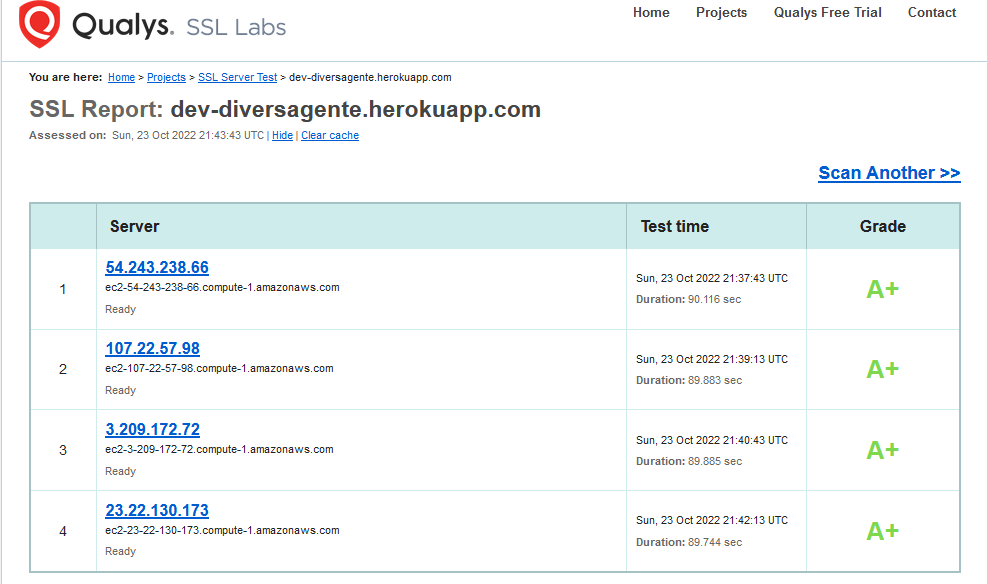
\includegraphics[width=0.90\textwidth]{anexos/SSLlabsII.png}
	\label{SSLLabsII}
	\fonte{Qualys SSL Labs, 2022 }
\end{figure}

\pagebreak

\section{Gitstats}

A ferramenta principal para o versionamento de código utilizada pela equipe de desenvolvimento é o \waUrlTitle{https://github.com/
}{GitHub}, e por meio do Gitstats foram geradas métricas gerais, das atividades, dos autores, dos arquivos e das tags no repositório. Para o desenvolvimento da parte I, todas as respectivas imagens das métricas podem ser encontradas dentro do \autoref{gisStatsI} e para a para uma análise mais completa, o 
\href{https://dev-diversagente.herokuapp.com/public/gitstats/}{Gitstats} é encontrado dentro no link: https://dev-diversagente.herokuapp.com/public/gitstats/


Nas métricas gerais do projeto \autoref{metricas1PartII}, a branch analisada consta como a gitstats, a qual já conta com mais de 863 commits dos sete integrantes do grupo no projeto diversaGente um aumento de cerca de 500 commits, e esses commits abarcam os trabalhos feitos desde a fundação dos projetos back-end e front-end mobile, além da organização da documentação LaTeX. 

\begin{figure}[htb]
	\centering
	\caption{\label{fig_arq_virado}Gitstats métricas gerais Parte II}
	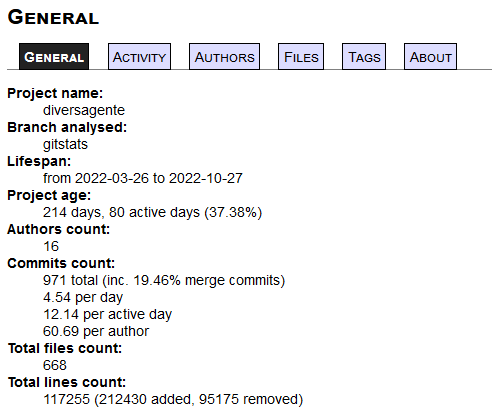
\includegraphics[width=1.00\textwidth]{anexos/metricas1PartII.png}
	\label{metricas1PartII}
	\fonte{Gitstats, 2022}
\end{figure}

\pagebreak

\begin{itemize}

\end{itemize}

Na aba de atividades \autoref{metricas2PartII}, são encontrados gráficos acerca da frequência dos commits realizados no projeto. É possível obter uma visualização em gráfico por mês do ano e horas por semana, por exemplo, evidenciando picos de trabalho durante o período de 365 dias da existência do projeto.

\begin{figure}[htb]
	\centering
	\caption{\label{fig_arq_virado}Gitstats métricas atividades Parte II}
	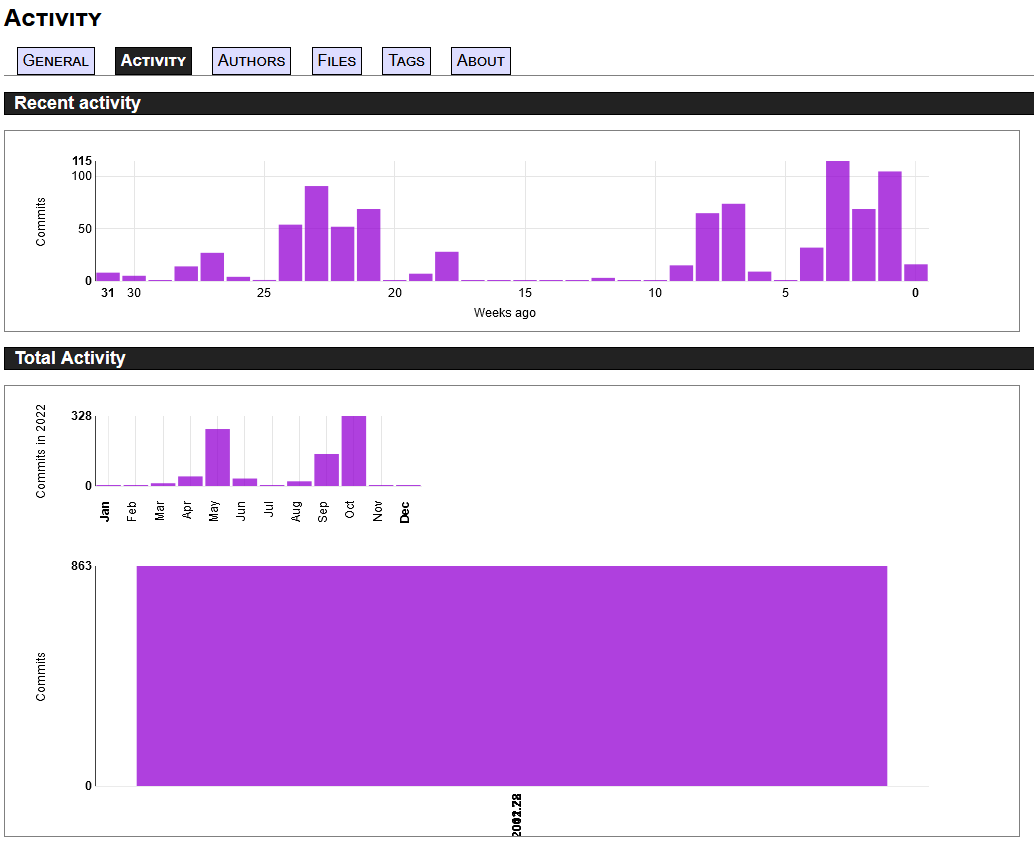
\includegraphics[width=0.90\textwidth]{anexos/metricas2PartII.png}
	\label{metricas2PartII}
	\fonte{Gitstats, 2022}
\end{figure}

Esse indicador demonstra \autoref{metricas3PartII} os autores mais ativos no projeto ao longo de sua existência. Devido as preparações para as demonstrações de \ac{poc} e \ac{mvp} e projeto final durante o ano, atuaram de forma mais intensa os que tinham um pouco mais de experiência com desenvolvimento, mas todos puderam contribuir para a entrega do projeto como um todo. 

\begin{figure}[htb]
	\centering
	\caption{\label{fig_arq_virado}Gitstats métricas autores Parte II}
	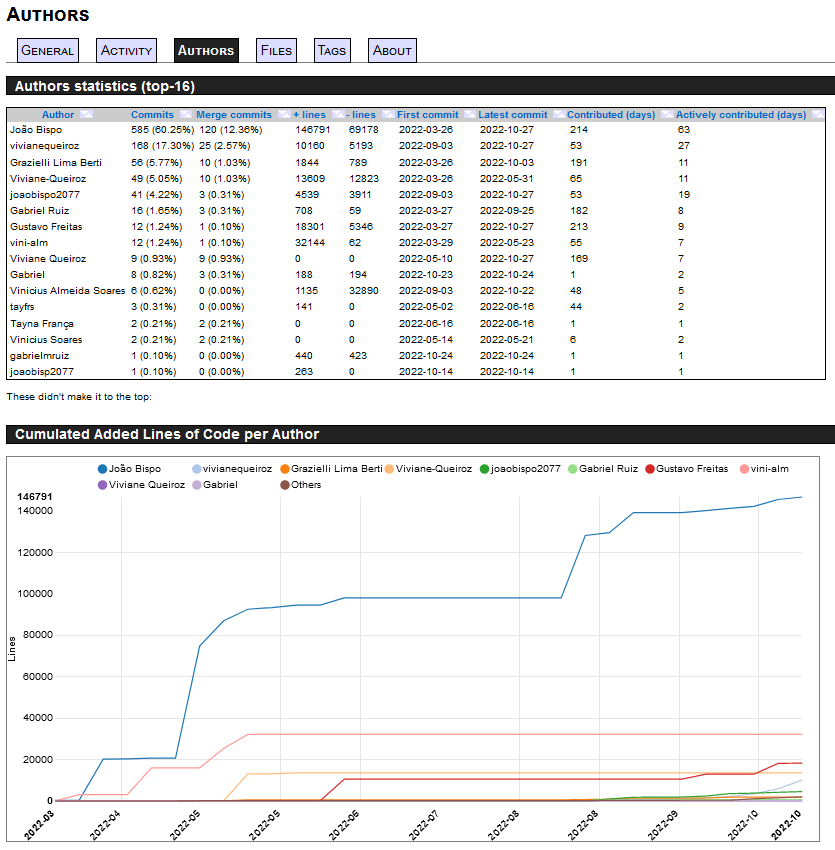
\includegraphics[width=1.00\textwidth]{anexos/metricas3PartII.png}
	\label{metricas3PartII}
	\fonte{Gitstats, 2022}
\end{figure}

Com essa métrica  \autoref{metricas4PartII}, é possível constatar que atualmente a base de códigos do projeto possui tamanho de 29.6 \ac{mb}, 637 arquivos no total, sendo os arquivos do tipo typescript os mais presentes em todo o projeto. 

\pagebreak



No momento, o projeto consta com apenas uma única tag \autoref{metricas5PartII}. Mas com o foco maior na parte de desenvolvimento da aplicação no próximo semestre, a quantidade de tags tende a aumentar progressivamente.


\begin{figure}[htb]
	\centering
	\caption{\label{fig_arq_virado}Gitstats métricas arquivos Parte II}
	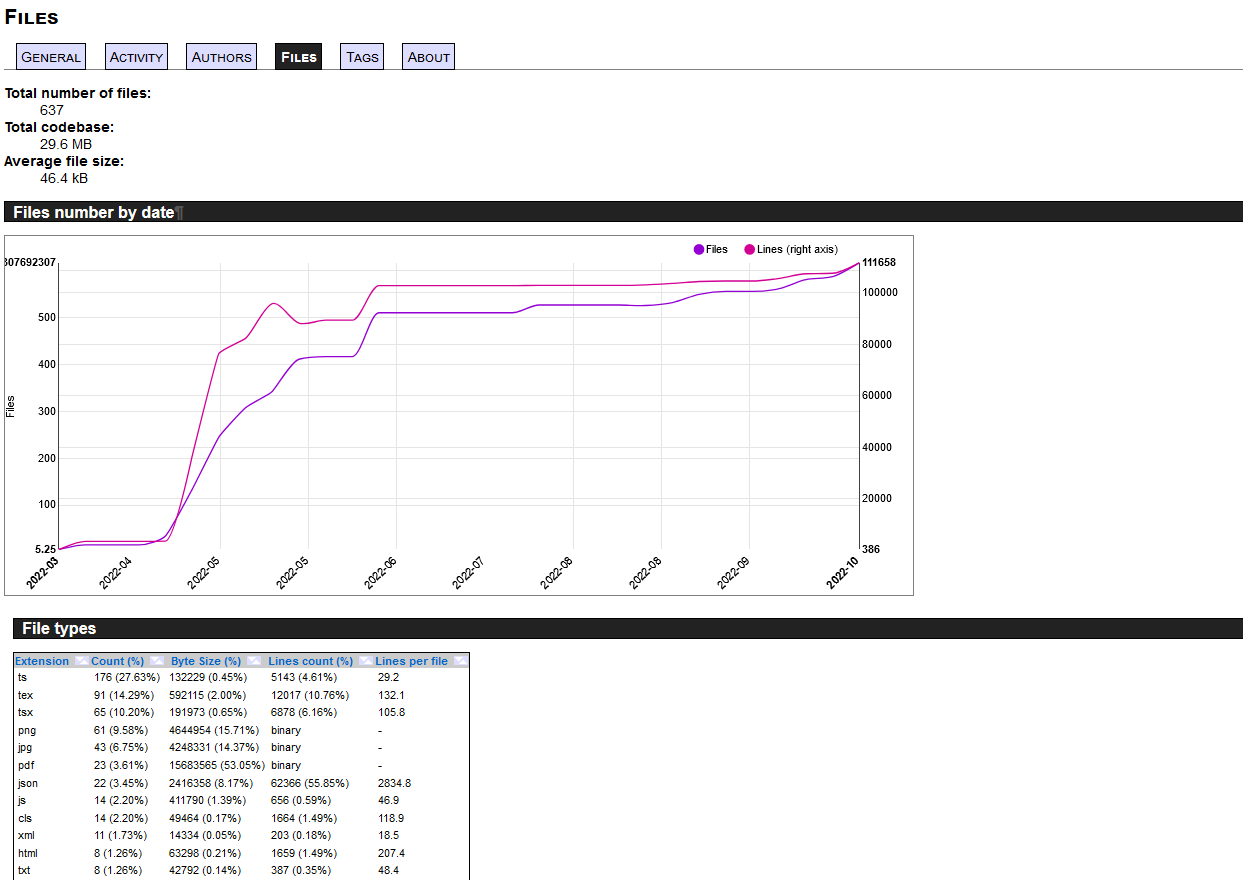
\includegraphics[width=1.00\textwidth]{anexos/metricas4PartII.png}
	\label{metricas4PartII}
	\fonte{Gitstats, 2022}
\end{figure}

\begin{figure}[htb]
	\centering
	\caption{\label{fig_arq_virado}Gitstats tags Parte II }
	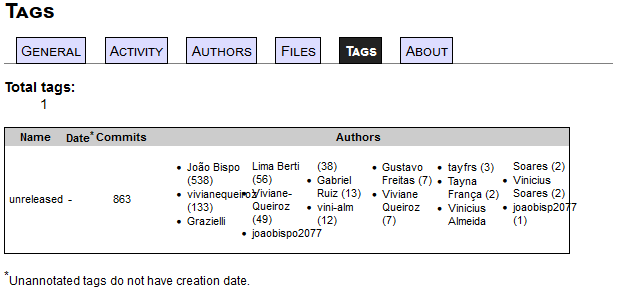
\includegraphics[width=1.00\textwidth]{anexos/metricas5PartII.png}
	\label{metricas5PartII}
	\fonte{Gitstats, 2022}
\end{figure}